%======================================================================
\chapter{AI Component Design}
%======================================================================

This chapter describes how Artificial Intelligence (AI) components are designed and
integrated into the overall system. Each section starts with a clear objective and provides
guidance on analysis, design, implementation, and evaluation of AI modules.

%------------------------------
\section{Business Context and AI Integration}
%------------------------------

\begin{figure}[htbp]
	\centering
	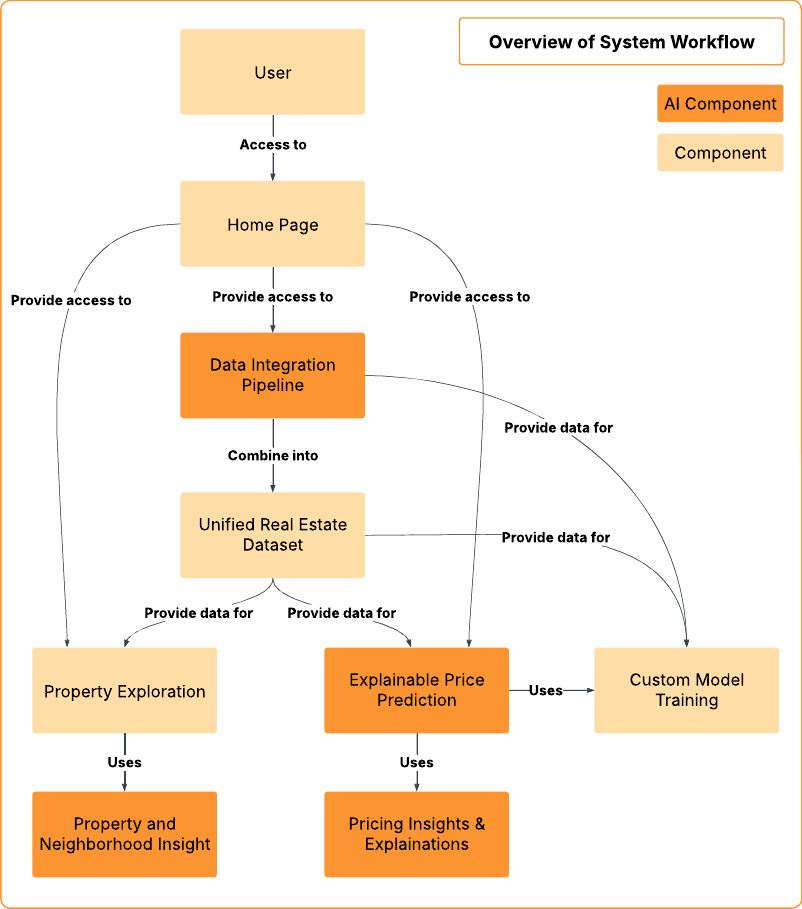
\includegraphics[width=1\textwidth]{assets/system-workflow.png}
	\caption{Overview system workflow}
	\label{fig:system-workflow}
\end{figure}

Figure~\ref{fig:system-workflow} shows the overview of the system workflow and how each component works together. It illustrates that AI will be used in four components: Data Integration Pipeline, Explainable Price Prediction, Property and Neighborhood Insight, and Pricing Explanation.

For each component, I will explain why using AI is both feasible and necessary.

\subsection*{1. Data Integration Pipeline}
Using AI is suitable in this case because content on websites varies by type of information and other elements, so AI needs to be implemented to help parse and understand the context and extract information.

When aggregating multiple data sources, differences in data schemas present a significant challenge. We need to establish a centralized data schema, and AI can help users accomplish this more easily by suggesting related fields.

For web scraping, the problem is complex and constantly changing because website structures vary across multiple sites and are difficult to parse with fixed rules. For file and API sources, the challenge is less complex since we can extract data from files and fetch data from API endpoints directly. However, complexity increases when combining these sources into one unified pipeline.

We can accept some incompleteness in this module. Missing fields in the aggregated data will not significantly affect the analysis when working with large volumes of data.

\subsection*{2. Explainable Price Prediction}
AI is appropriate for price prediction because housing prices are influenced by numerous factors that interact in complex, non-linear ways. Traditional rule-based systems cannot effectively capture these intricate relationships.

The housing market constantly evolves with changing economic conditions, buyer preferences, and seasonal variations. AI models can adapt to these shifts by identifying new patterns in the data that might not be obvious to human analysts.

We can accept predictions that are not 100\% accurate since real estate valuation inherently involves some uncertainty. However, by using explainable AI approaches, we can provide confidence intervals and explain the key factors influencing each prediction, making the system valuable even with some margin of error.

\subsection*{3. Property and Neighborhood Insight}
AI is well-suited for generating property and neighborhood insights because this requires analyzing diverse data types including text descriptions, images, geographic information, and numerical data. The relationships between these varied data sources are complex and difficult to codify with traditional rules.

The characteristics that make a neighborhood desirable change over time and vary across different buyer segments. AI can identify emerging trends and personalized insights that static analysis would miss.

Perfect completeness is not essential, as providing valuable insights on the most significant factors affecting property desirability is more important than capturing every minor detail. Users benefit from focused, relevant information rather than exhaustive analysis.

\subsection*{4. Pricing Explanation}
Using AI for pricing explanation is appropriate because explaining property valuations involves communicating complex relationships between numerous factors in an accessible way. These explanations need to adapt to each property's unique characteristics and the specific market context.

The relative importance of different pricing factors changes across markets and over time. AI can generate contextual explanations that reflect these dynamics rather than relying on fixed templates.

While we can accept explanations that might not cover every possible factor influencing price, the system provides significant value by highlighting the most important considerations and presenting them in a clear, understandable format for users.

\newpage

%------------------------------
\section{Goal Hierarchy}
%------------------------------

This section outlines the hierarchical structure of goals for our real estate valuation system, beginning with organizational objectives and flowing down to specific AI model goals. For each level, We provide clear metrics to measure success.

\subsection{Organizational Goals}

The primary organizational goals for this AI system are:

\begin{itemize}
	\item To establish a trusted platform for accurate and transparent real estate valuations
	\item To build a reputation for innovation in applying AI to real estate challenges
\end{itemize}

Success at the organizational level will be measured through:

\begin{itemize}
	\item Recognition through awards
\end{itemize}

\subsection{System Goals}

At the system level, our goals are:

\begin{itemize}
	\item To integrate diverse real estate data sources into a unified, high-quality dataset
	\item To generate accurate property valuations with clear explanations for price factors
	\item To provide insightful property and neighborhood analysis to inform decision-making
	\item To deliver a reliable, responsive user experience across different devices and user types
\end{itemize}

System success metrics include:

\begin{itemize}
	\item System uptime and response time statistics
	\item Data completeness and quality indicators across different property types and regions
	\item System error rates and exception handling effectiveness
	\item System scalability under increasing data volumes and user numbers
\end{itemize}

\subsection{User Goals}

For our users, the goals are:

\begin{itemize}
	\item To receive insightful property valuations they can trust for decision-making
	\item To understand the key factors influencing property prices in specific markets
	\item To gain insights about properties and neighborhoods beyond basic statistics
	\item To save time in researching and analyzing real estate opportunities
\end{itemize}

User success metrics will be assessed through:

\begin{itemize}
	\item User satisfaction surveys and net promoter scores
\end{itemize}

\subsection{AI Model Goals}

At the most specific level, our AI model goals are:

\begin{itemize}
	\item To accurately predict property prices with clearly quantified confidence levels
	\item To identify and weigh the most influential factors affecting property values
	\item To provide explanations for predictions that are both technically sound and accessible to non-technical users
\end{itemize}

AI model performance will be measured through:

\begin{itemize}
	\item Statistical accuracy metrics including mean absolute error, root mean squared error, and R-squared value compared to actual transaction prices
	\item Explanation quality assessed through user comprehension testing
	\item Comparative performance against benchmark models and traditional valuation methods
	\item Drift detection metrics to identify when model retraining is necessary
	\item Computational efficiency metrics including inference time and resource utilization
\end{itemize}

%------------------------------
\section{Task Requirements Analysis Using AI Canvas}
%------------------------------

This section presents a detailed analysis of our AI system's task requirements using the AI Canvas methodology. This approach helps us clearly articulate what each AI component should accomplish, how it will operate technically, and the conditions under which it will function.

\subsection{AI Task Requirements}
For each AI component in our system, we analyze three key dimensions:
\begin{itemize}
	\item \textbf{Requirements (REQ):} The specific objectives and functions each AI component must fulfill
	\item \textbf{Specifications (SPEC):} The technical approach and methods the AI will employ
	\item \textbf{Environment (ENV):} The operational conditions, constraints, and context in which the AI will function
\end{itemize}

\subsubsection*{1. Data Integration Pipeline}

\textbf{Requirements (REQ):} The AI component must extract structured data from diverse sources including property listing websites, government databases, and unstructured documents. It needs to identify property characteristics, pricing information, location data, and temporal attributes across varying formats. The system must normalize extracted data into a unified schema.

\textbf{Specifications (SPEC):} This component will implement a hybrid approach combining rule-based extraction for standardized sources and deep learning models for unstructured content. Named entity recognition models will identify property attributes within text, while transformer-based architectures will handle context-dependent extraction tasks.

\textbf{Environment (ENV):} The component will operate in a data environment characterized by high heterogeneity across sources, frequent changes in website structures, and varying data quality. It must process large volumes of daily updates while maintaining extraction accuracy. The system requires periodic retraining as new data sources are integrated and reasonable human oversight for exception handling of complex cases that fall outside standard patterns.

\subsubsection*{2. Explainable Price Prediction}

\textbf{Requirements (REQ):} This AI component must generate accurate property valuation estimates with quantified confidence intervals. It needs to identify key value drivers specific to each property, adapt to regional market dynamics, and provide predictions that remain reliable even with incomplete input data. The system must detect when it lacks sufficient information for reliable prediction and communicate these limitations transparently.

\textbf{Specifications (SPEC):} The prediction engine will utilize an ensemble approach combining gradient-boosted decision trees for tabular data with graph neural networks to capture neighborhood relationships and spatial dependencies. SHAP values and counterfactual explanations will provide feature importance analysis.

\textbf{Environment (ENV):} This component operates within a complex market environment.

\subsubsection*{3. Property and Neighborhood Insight}

\textbf{Requirements (REQ):} The AI must analyze multilayered neighborhood data to identify significant patterns and trends relevant to property valuation. It needs to generate insights about local amenities, infrastructure developments, community characteristics, and future growth potential.

\textbf{Specifications (SPEC):} This component will utilize multimodal analysis techniques combining geospatial machine learning for location-based features with natural language processing for textual descriptions and sentiment analysis. The system will implement clustering algorithms to identify comparable neighborhoods and temporal modeling to detect emerging trends.

\textbf{Environment (ENV):} The insight generation occurs in an information-rich but fragmented environment with data spanning multiple domains including transportation, education, commerce, and safety. The component must operate with varying data availability across neighborhoods and maintain cultural sensitivity when analyzing community characteristics. It needs to distinguish between transient and persistent neighborhood attributes while balancing detail with relevance in its output.

\subsubsection*{4. Pricing Explanation}

\textbf{Requirements (REQ):} This component must translate complex valuation models into clear, intuitive explanations. It needs to communicate uncertainty appropriately, highlight the most influential factors affecting a specific property's value, and provide comparative analysis with similar properties. The system should generate explanations that help users understand market dynamics without overwhelming them with technical details.

\textbf{Specifications (SPEC):} The explanation system will implement a natural language generation pipeline built on a large language model fine-tuned for real estate domain knowledge. It will incorporate techniques from the field of explainable AI including feature attribution visualization, importance ranking. The system will use templates for consistent structure while leveraging dynamic content generation for property-specific insights.

\textbf{Environment (ENV):} This component operates at the interface between technical prediction systems and non-technical users.

\newpage

\subsection{AI Canvas Development}

\subsubsection{1. Data schema mapping}

\begin{figure}[htbp]
	\centering
	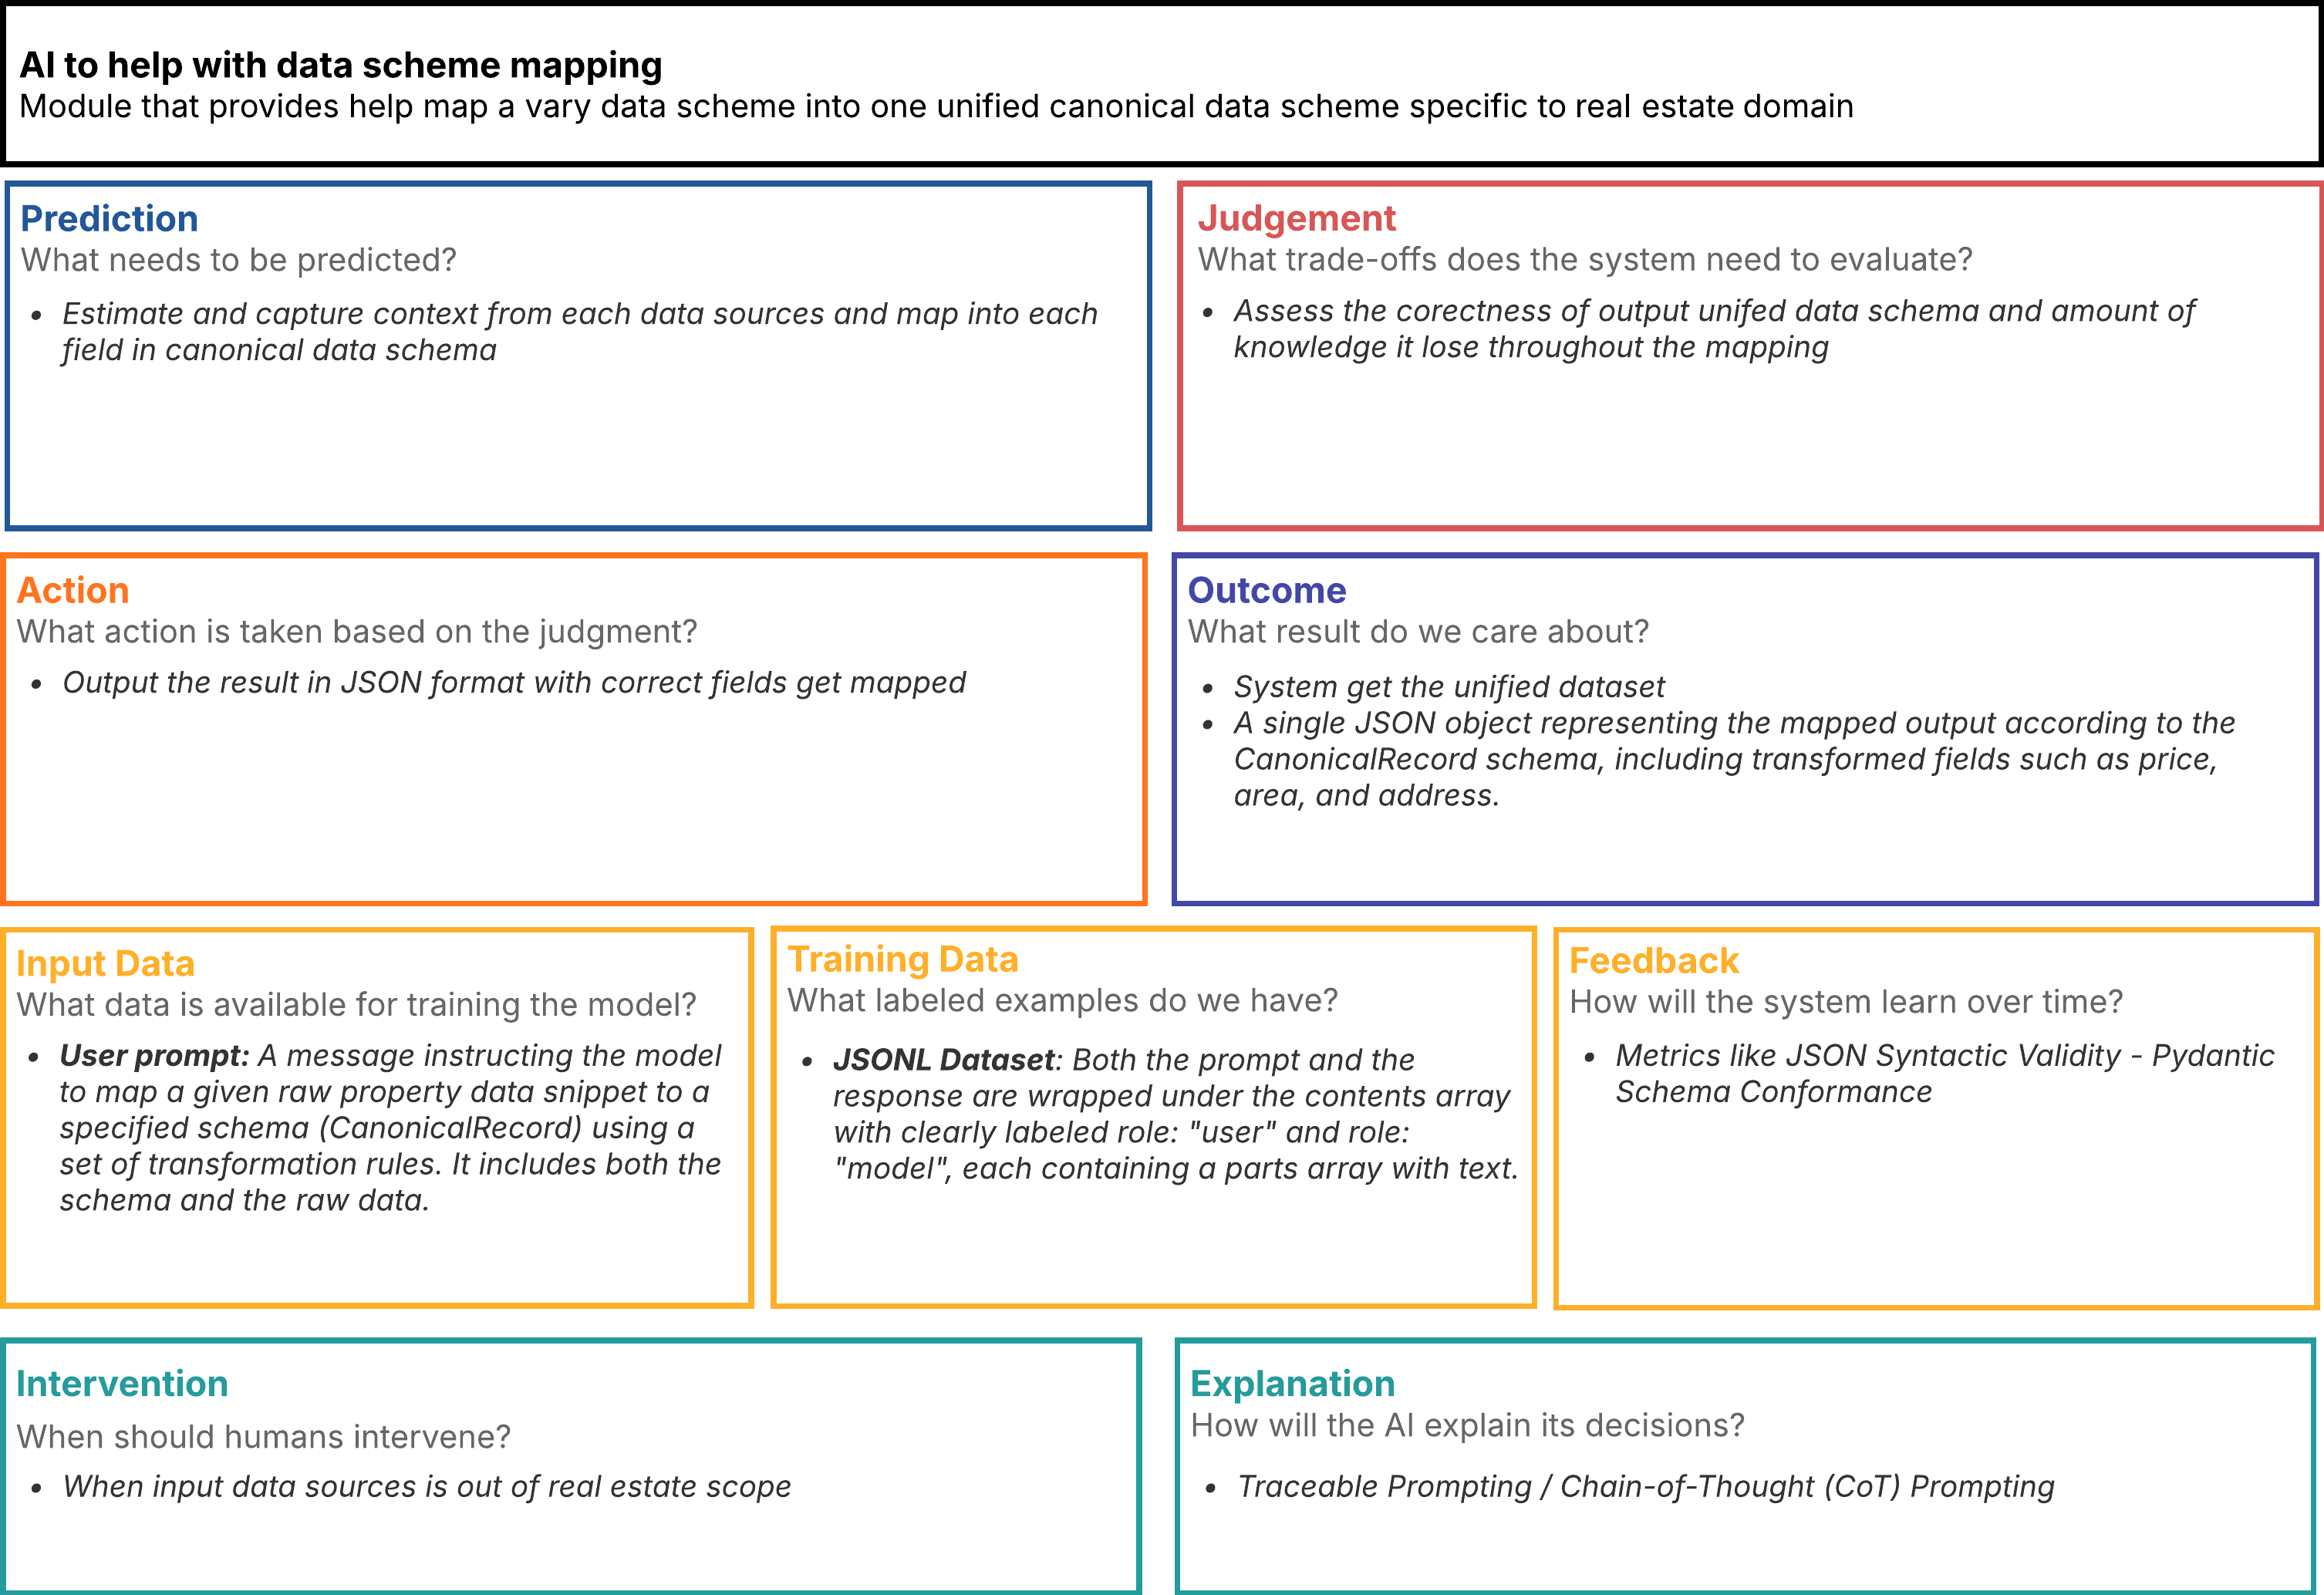
\includegraphics[width=1\textwidth]{assets/ai/ai-canvas-2.png}
	\caption{Data schema mapping AI Canvas}
	\label{fig:ai-canvas-1}
\end{figure}

\noindent Figure \ref{fig:ai-canvas-1} presents an AI Canvas diagram for a Real Estate Data Schema Mapping system. This strategic planning tool articulates how artificial intelligence creates value through structured components that guide the implementation of a unified canonical data schema for real estate information.

The AI Canvas comprises eight interconnected sections that collectively define the system's purpose and operation. The Prediction section establishes the core functionality: estimating and capturing context from each data source and mapping it into each field in the canonical data schema. This works in concert with the Judgment section, which articulates the critical trade-offs the system must evaluate, focusing on assessing the correctness of the output unified data schema and measuring the amount of knowledge potentially lost throughout the mapping process.

The Action section defines how the system's outputs are translated into tangible steps, outputting the results in JSON format with correctly mapped fields. These actions lead to the Outcome section, which clarifies the ultimate value proposition: generating a unified dataset represented as a single JSON object conforming to the CanonicalRecord schema, including transformed fields such as price, area, and address.

The Input Data section catalogues the available information sources: user prompts containing instructions for mapping raw property data snippets to a specified schema (CanonicalRecord) using transformation rules, including both the schema specifications and the raw data itself. Complementing this, the Training Data section defines the labeled examples powering the model: JSONL datasets where both prompts and responses are wrapped in contents arrays with clearly labeled roles ("user" and "model"), each containing parts arrays with text.

The Feedback section outlines how the model will learn over time by tracking metrics like JSON Syntactic Validity and Pydantic Schema Conformance. The Intervention section establishes boundaries for human oversight, calling for expert involvement when input data sources fall outside the real estate scope. The Explanation section details the technical approaches for transparency: Traceable Prompting and Chain-of-Thought (CoT) Prompting methodologies to provide insight into the system's decision-making processes.


\subsubsection{2. Explainable Price Predition}

\begin{figure}[htbp]
	\centering
	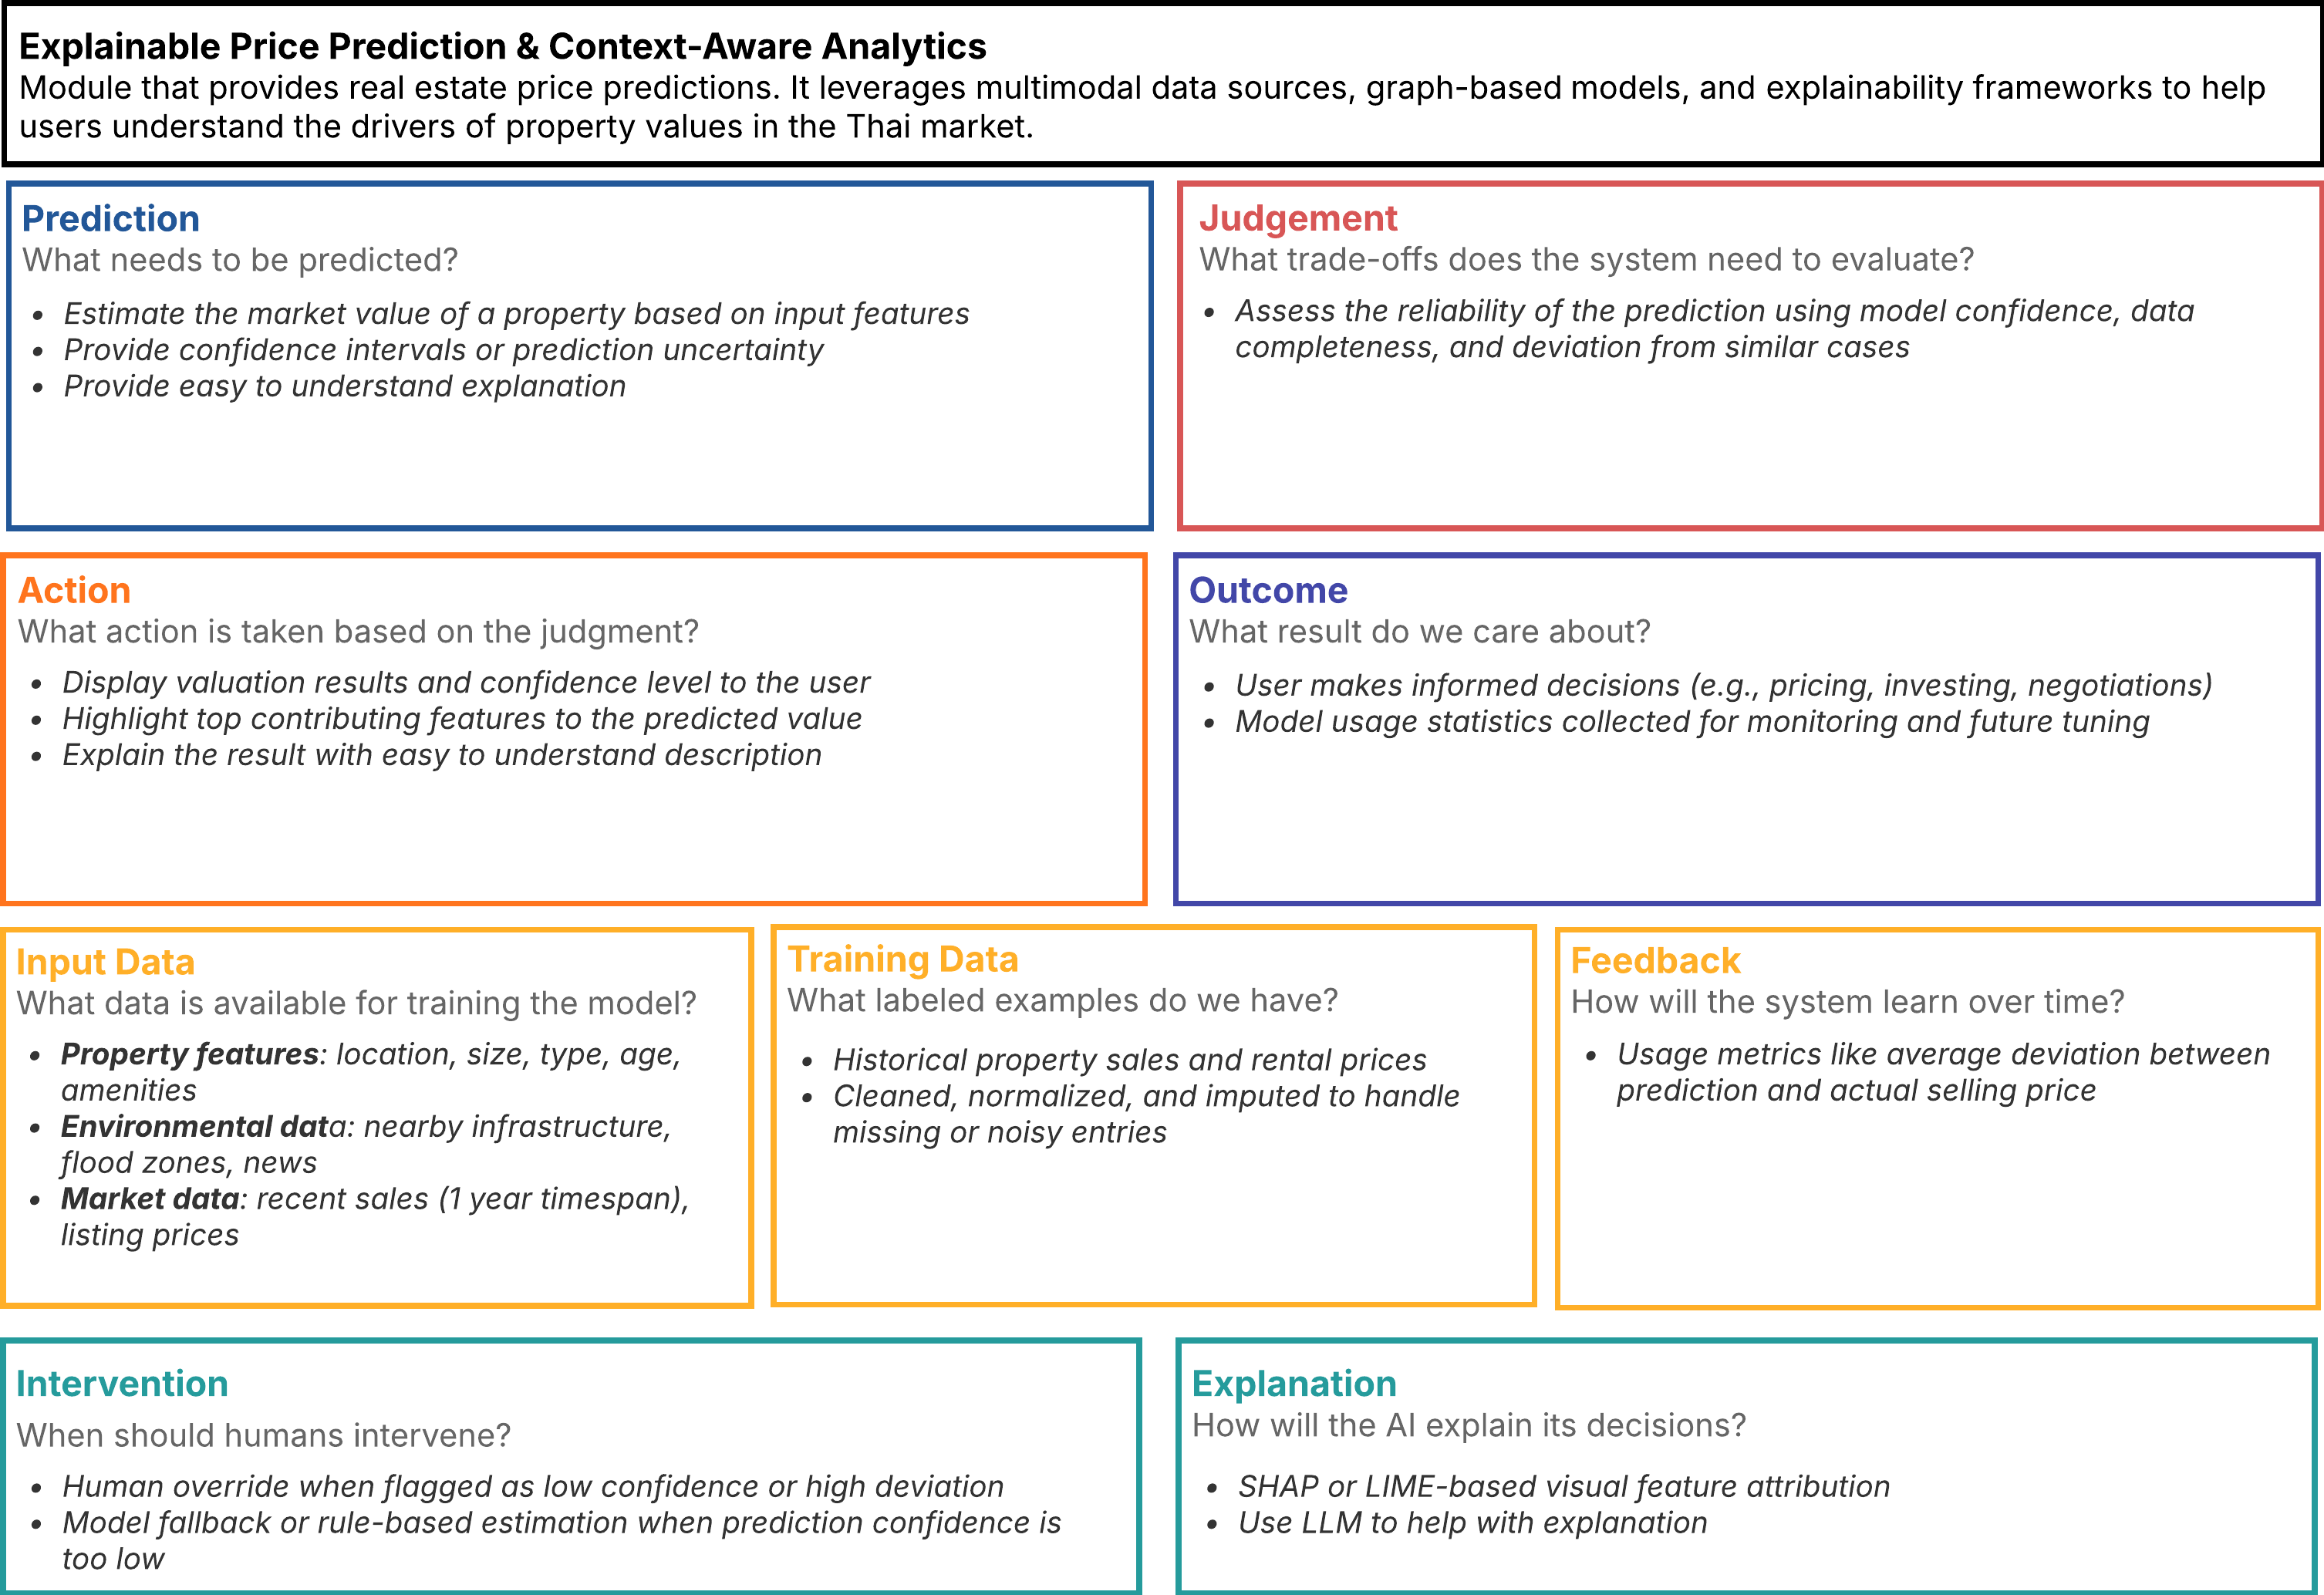
\includegraphics[width=1\textwidth]{assets/ai/ai-canvas.png}
	\caption{Explainable Price Predition AI Canvas}
	\label{fig:ai-canvas-2}
\end{figure}

\noindent Figure \ref{fig:ai-canvas-2} presents an AI Canvas diagram for an Explainable Price Prediction \& Context-Aware Analytics system tailored to the Thai real estate market. This strategic planning tool articulates how artificial intelligence creates value through structured components that guide implementation.

The AI Canvas comprises eight interconnected sections that collectively define the system's purpose and operation. The Prediction section establishes the core functionality: estimating property market values based on input features, providing confidence intervals to quantify uncertainty, and delivering accessible explanations to users. This works in concert with the Judgment section, which articulates the critical trade-offs the system must evaluate, focusing on assessing prediction reliability through model confidence metrics, data completeness evaluation, and deviation analysis from comparable properties.

The Action section defines how the system's outputs are translated into tangible steps, displaying valuation results with confidence levels, highlighting the top contributing features to predicted values, and explaining results through user-friendly descriptions. These actions lead to the Outcome section, which clarifies the ultimate value proposition: enabling users to make informed real estate decisions across pricing, investing, and negotiations, while simultaneously collecting usage statistics for ongoing system optimization.

The Input Data section catalogues the available information sources: property features including location, size, type, age, and amenities; environmental data encompassing infrastructure, flood zones, and news; and market data covering recent sales and current listings. Complementing this, the Training Data section defines the labeled examples powering the model: historical sales and rental prices that have undergone cleaning, normalization, and imputation processes to handle data quality issues.

The Feedback section outlines how the model will learn over time by tracking metrics like average deviation between predictions and actual selling prices. The Intervention section establishes boundaries for human oversight, calling for expert involvement when predictions show low confidence or high deviation, while implementing fallback mechanisms when prediction certainty falls below acceptable thresholds. The Explanation section details the technical approaches for transparency: SHAP or LIME-based visual feature attribution combined with Large Language Models to generate intuitive explanations.

\newpage


\newpage

%------------------------------
\section{User Experience Design with AI}
%------------------------------

This section explains how AI is used to improve the user experience in our real estate system. AI is not just a background tool—it helps users by doing tasks, adding helpful info, giving smart suggestions, and adjusting to user needs. These features are built into key parts of the system, like data handling, neighborhood analysis, and price prediction. The design focuses on being clear, easy to use, and useful for different types of users.

\subsection{Automated Pipelines}

The pipeline system in BorBann is not just a backend tool. It’s a dynamic, AI interface that enables even non-technical users to build, manage, and leverage data workflows for training personalized real estate models.

The system is designed using an \textbf{Automate} style that automatically handles repetitive technical tasks—like schema inference and spider generation—but still gives users the power to manually adjust the process.

\subsubsection*{1. Pipeline Creation and Management}

Users start by selecting data sources—like websites, files, or APIs—and use a no-code interface to configure their pipeline. The system generates scraping rules using an LLM and recommends schema alignments automatically.

\begin{figure}[htbp]
	\centering
	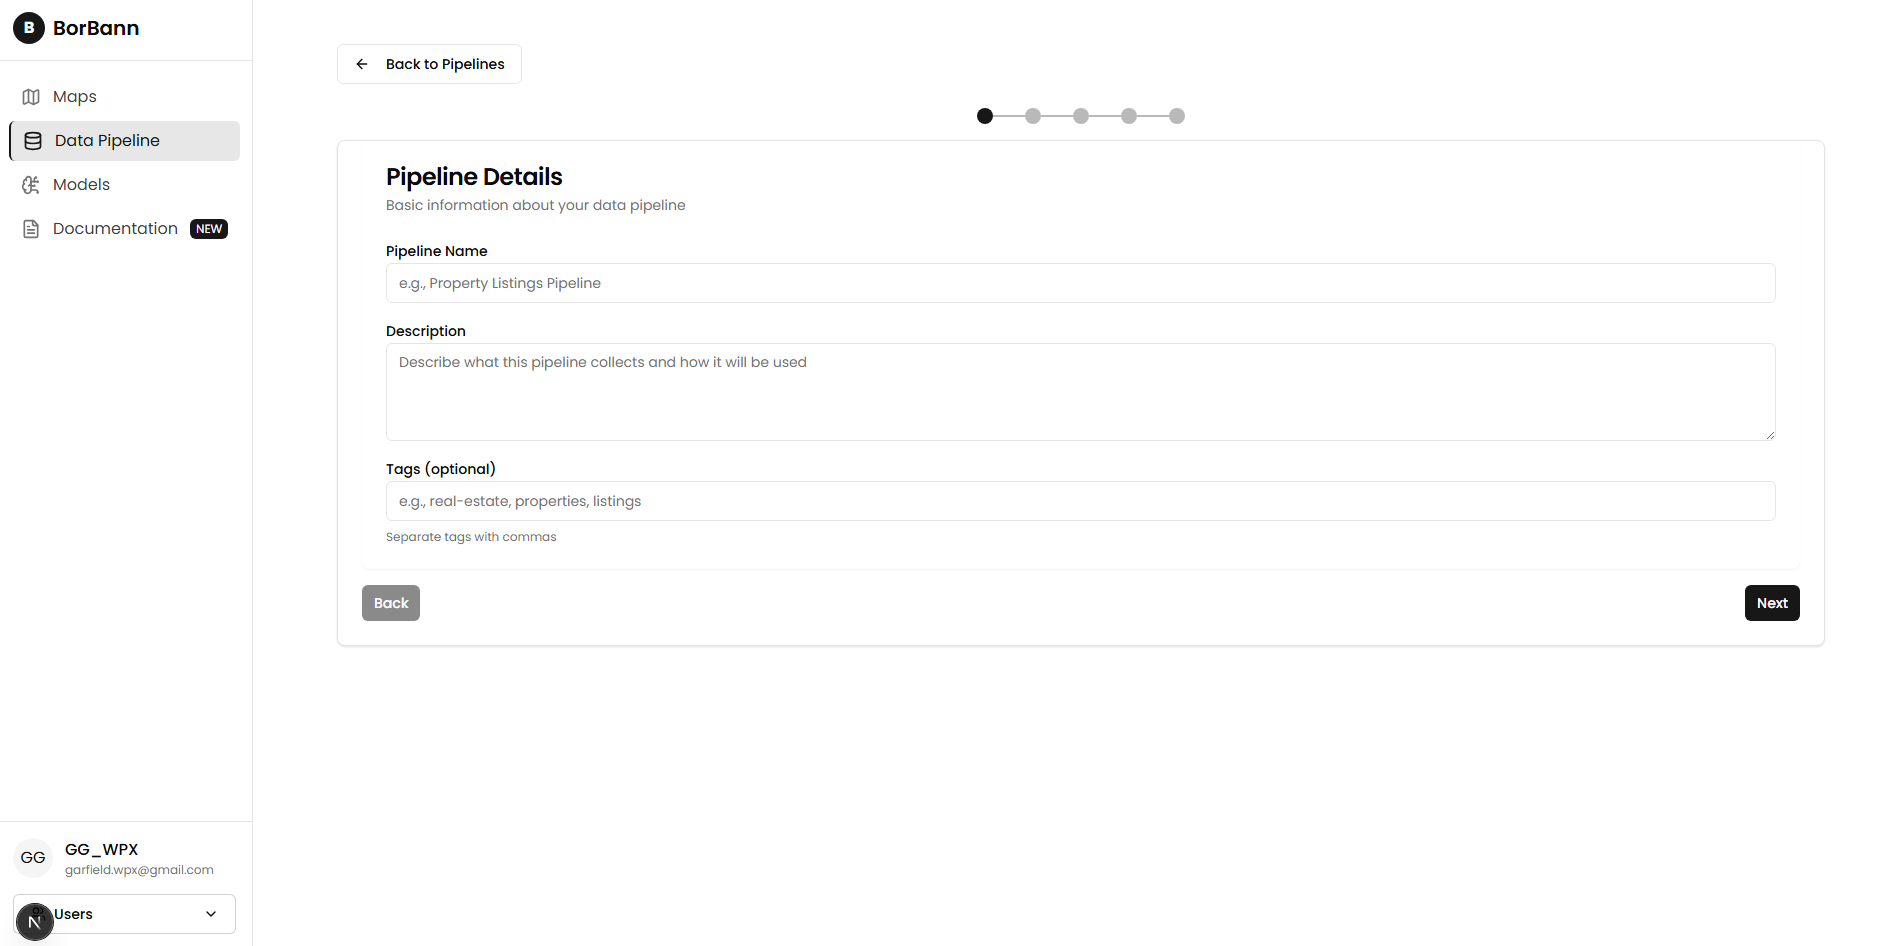
\includegraphics[width=1\textwidth]{assets/ai/pipeline-1.png}
	\caption{Pipeline Creation Interface}
	\label{fig:pipeline-creation-ui}
\end{figure}

\begin{figure}[htbp]
	\centering
	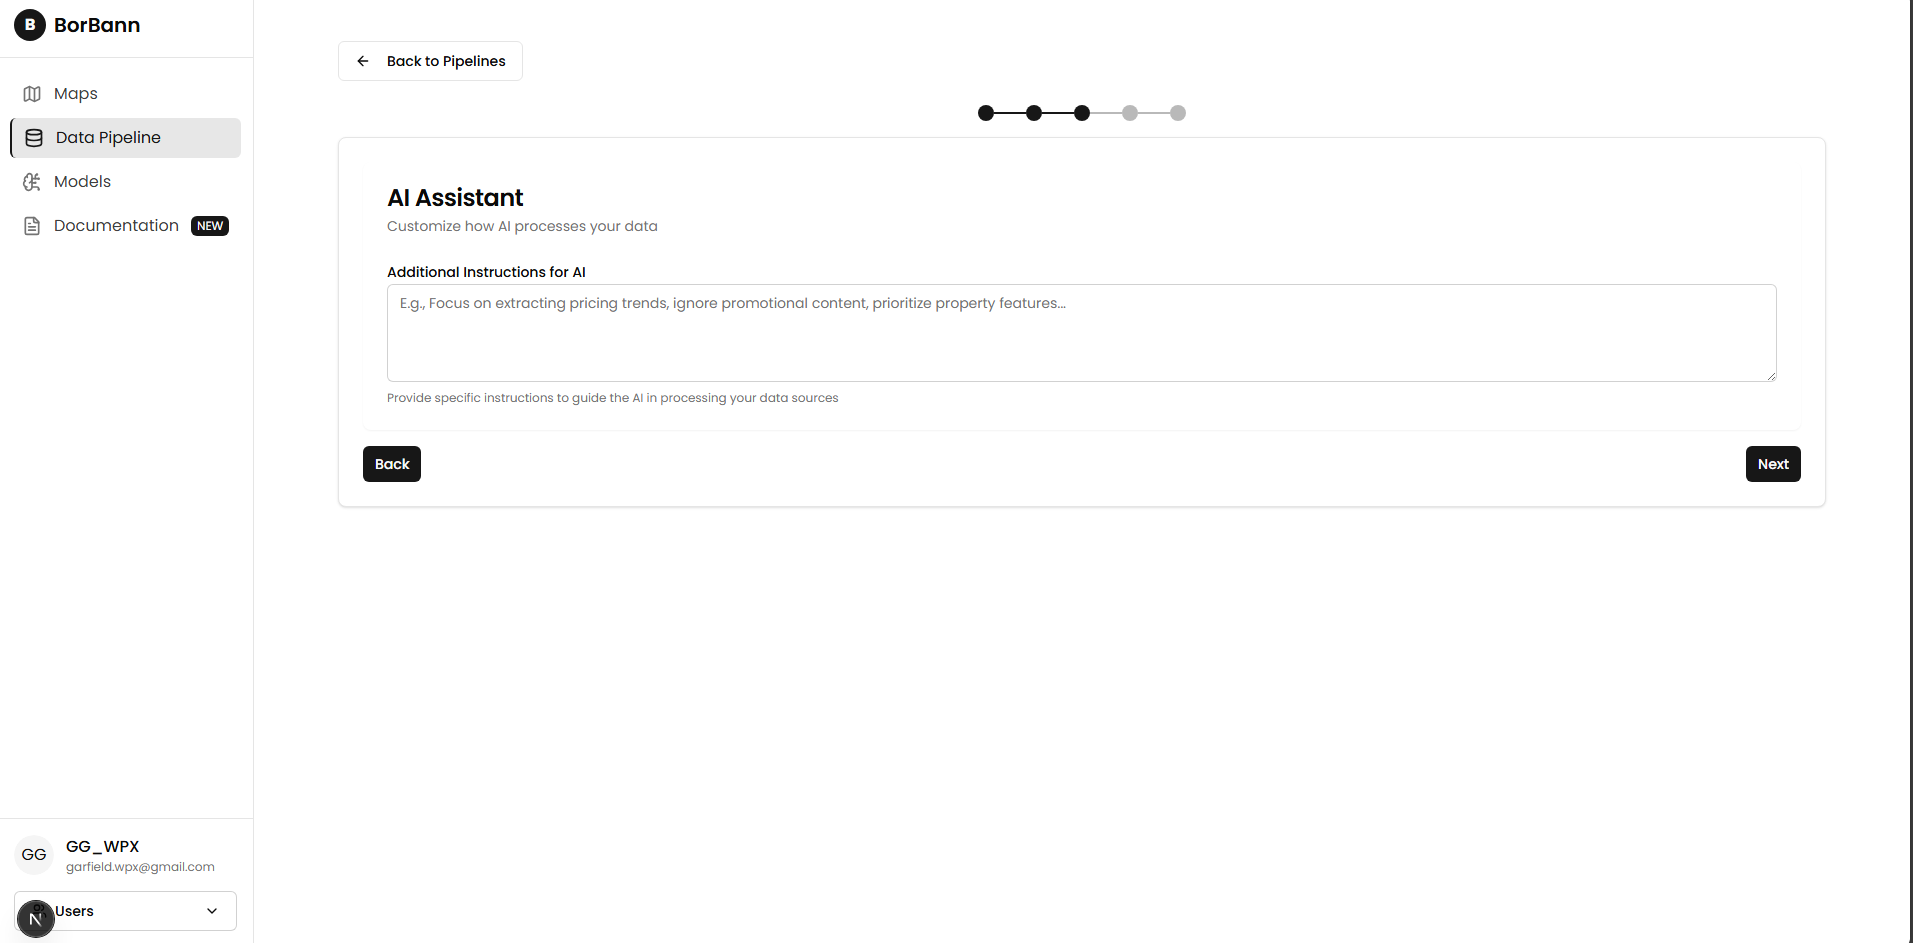
\includegraphics[width=1\textwidth]{assets/ai/pipeline-3.png}
	\caption{Pipeline Creation Interface – Additional Prompt}
	\label{fig:pipeline-creation-ui-2}
\end{figure}

Figures \ref{fig:pipeline-creation-ui} and \ref{fig:pipeline-creation-ui-2} show how users input data source URLs and set extraction options with help from the AI.

\subsubsection*{2. Field Customization and Schema Annotation}

After setting up the source, users can view, modify, or remove fields detected by the system. The interface visually maps fields across sources, includes data type validation, and supports custom field creation via formulas.

\begin{figure}[htbp]
	\centering
	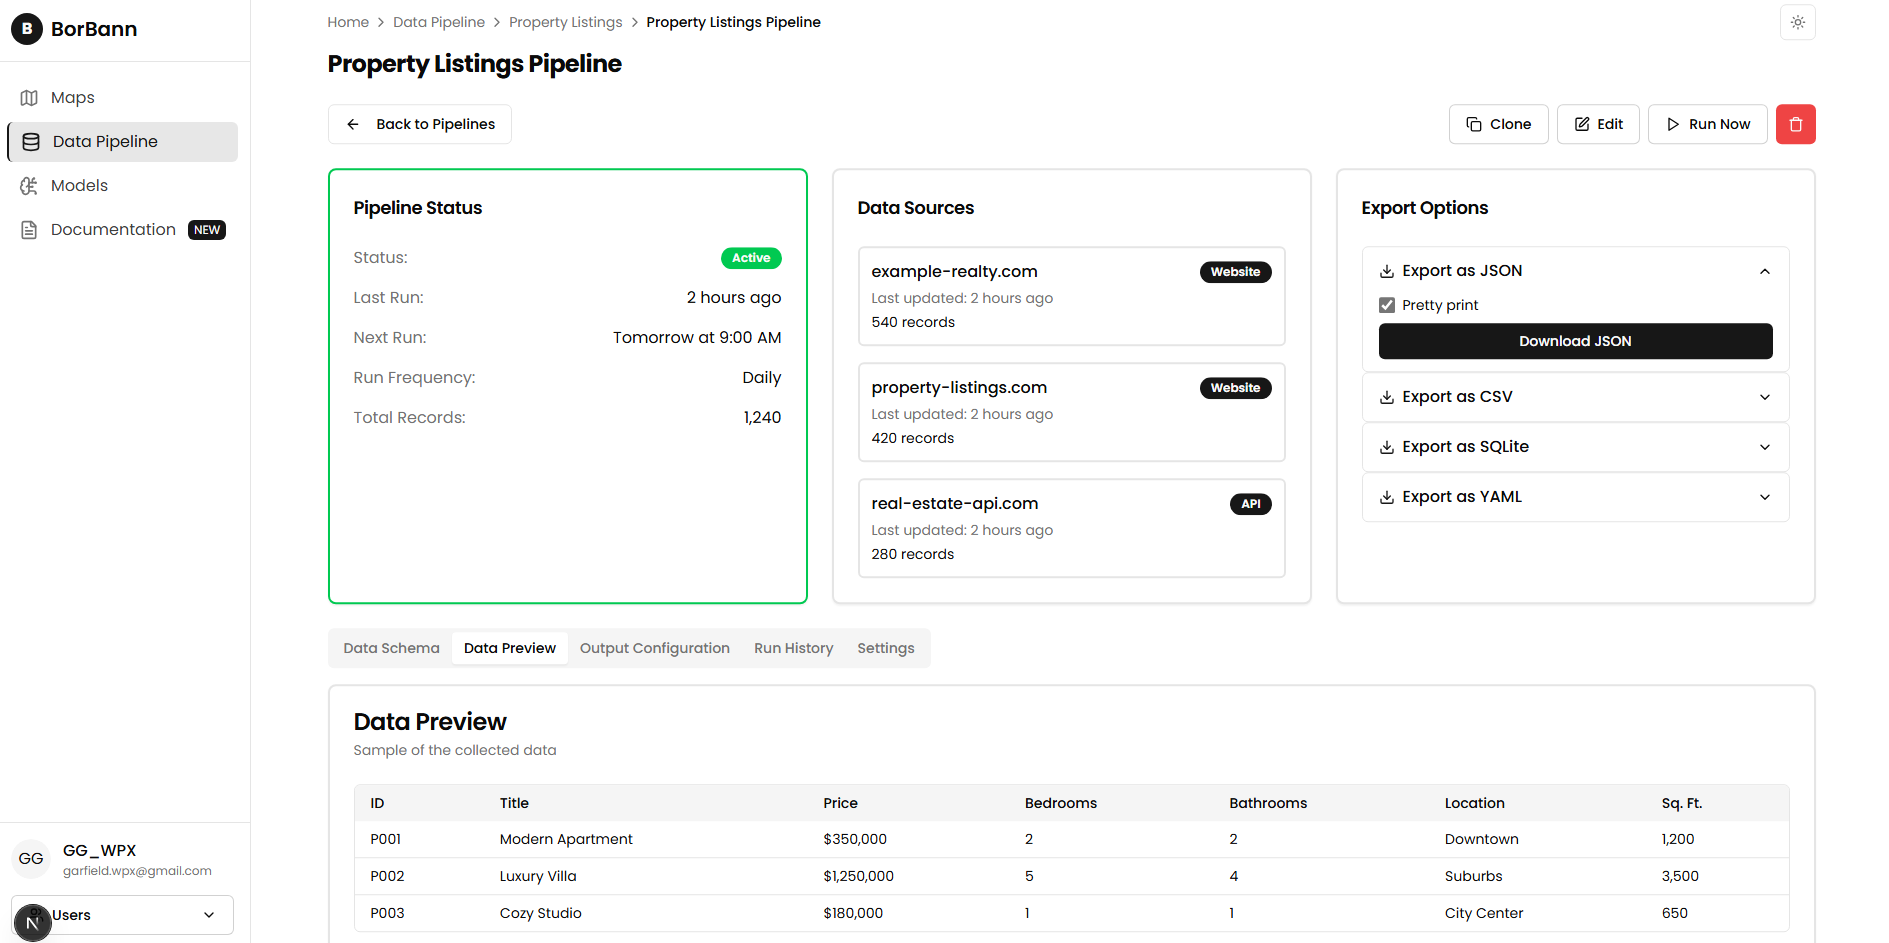
\includegraphics[width=1\textwidth]{assets/ai/pipeline-4.png}
	\caption{Field Management Interface}
	\label{fig:pipeline-creation-ui-3}
\end{figure}

Figure \ref{fig:pipeline-creation-ui-3} shows the functionalities to customize the schema and data source integration.

\subsubsection*{3. Pipeline Monitoring and Status Overview}

Users can view a dashboard that summarizes the status of each pipeline—categorized as Active, Paused, Failed, or Completed. Each pipeline card is annotated with insights.

\begin{figure}[htbp]
	\centering
	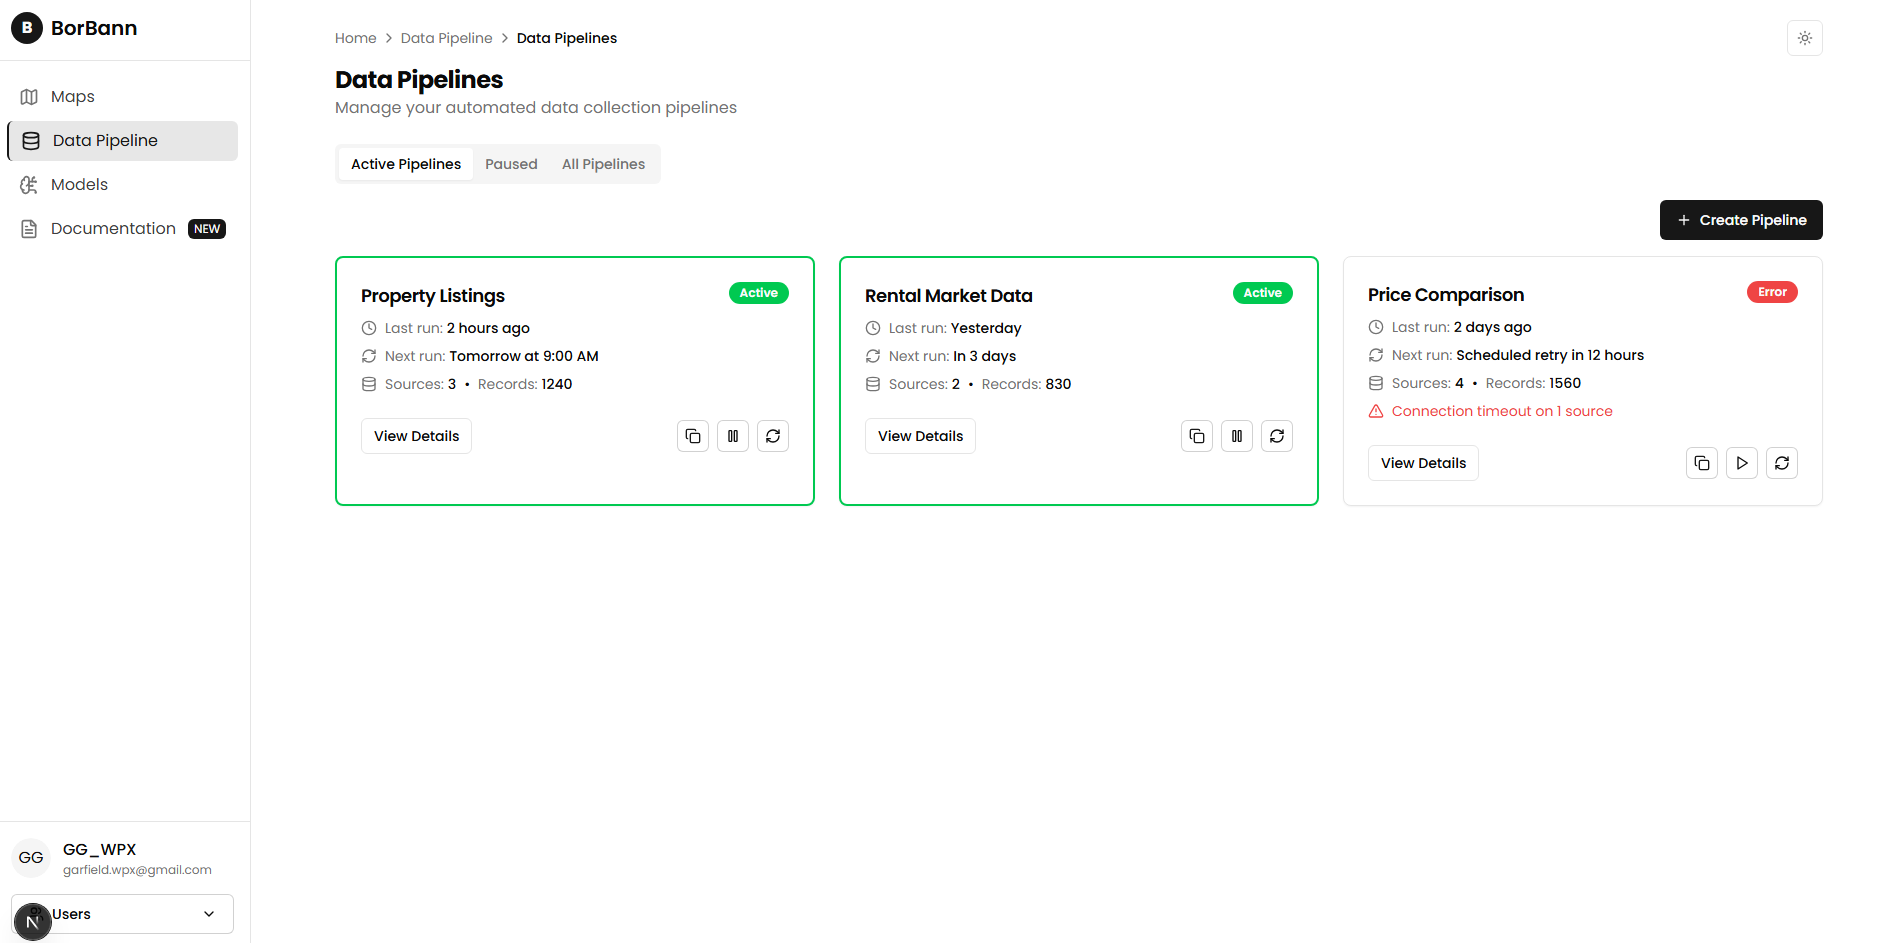
\includegraphics[width=1\textwidth]{assets/ai/pipeline-6.png}
	\caption{Pipeline Dashboard Interface}
	\label{fig:pipeline-creation-ui-4}
\end{figure}

Figure \ref{fig:pipeline-creation-ui-4} shows how the interface represents pipeline statuses; successful pipelines are highlighted with green-bordered cards.

\subsection{Neighborhood Insight}

The Neighborhood Insight feature uses various APIs and tools to analyze environmental conditions, nearby facilities, local amenities, and even news sentiment. The goal is to support smarter decisions by making the neighborhood story as transparent and rich as the property details.

This feature uses \textbf{Annotate}, which overlays real-time and historical context—like flood risk, school quality, and air pollution levels—into property views; and \textbf{Automate}, where the agent automatically pulls data from multiple sources and updates insights with minimal input.

\subsubsection*{1. Local Context Analytics Interface}

When users view a property, the system automatically presents key neighborhood metrics, including:

\begin{itemize}
	\item Flood risk history and air quality trends
	\item Distance and quality scores for nearby schools, hospitals, and transit points
	\item Local news sentiment
\end{itemize}

\begin{figure}[htbp]
	\centering
	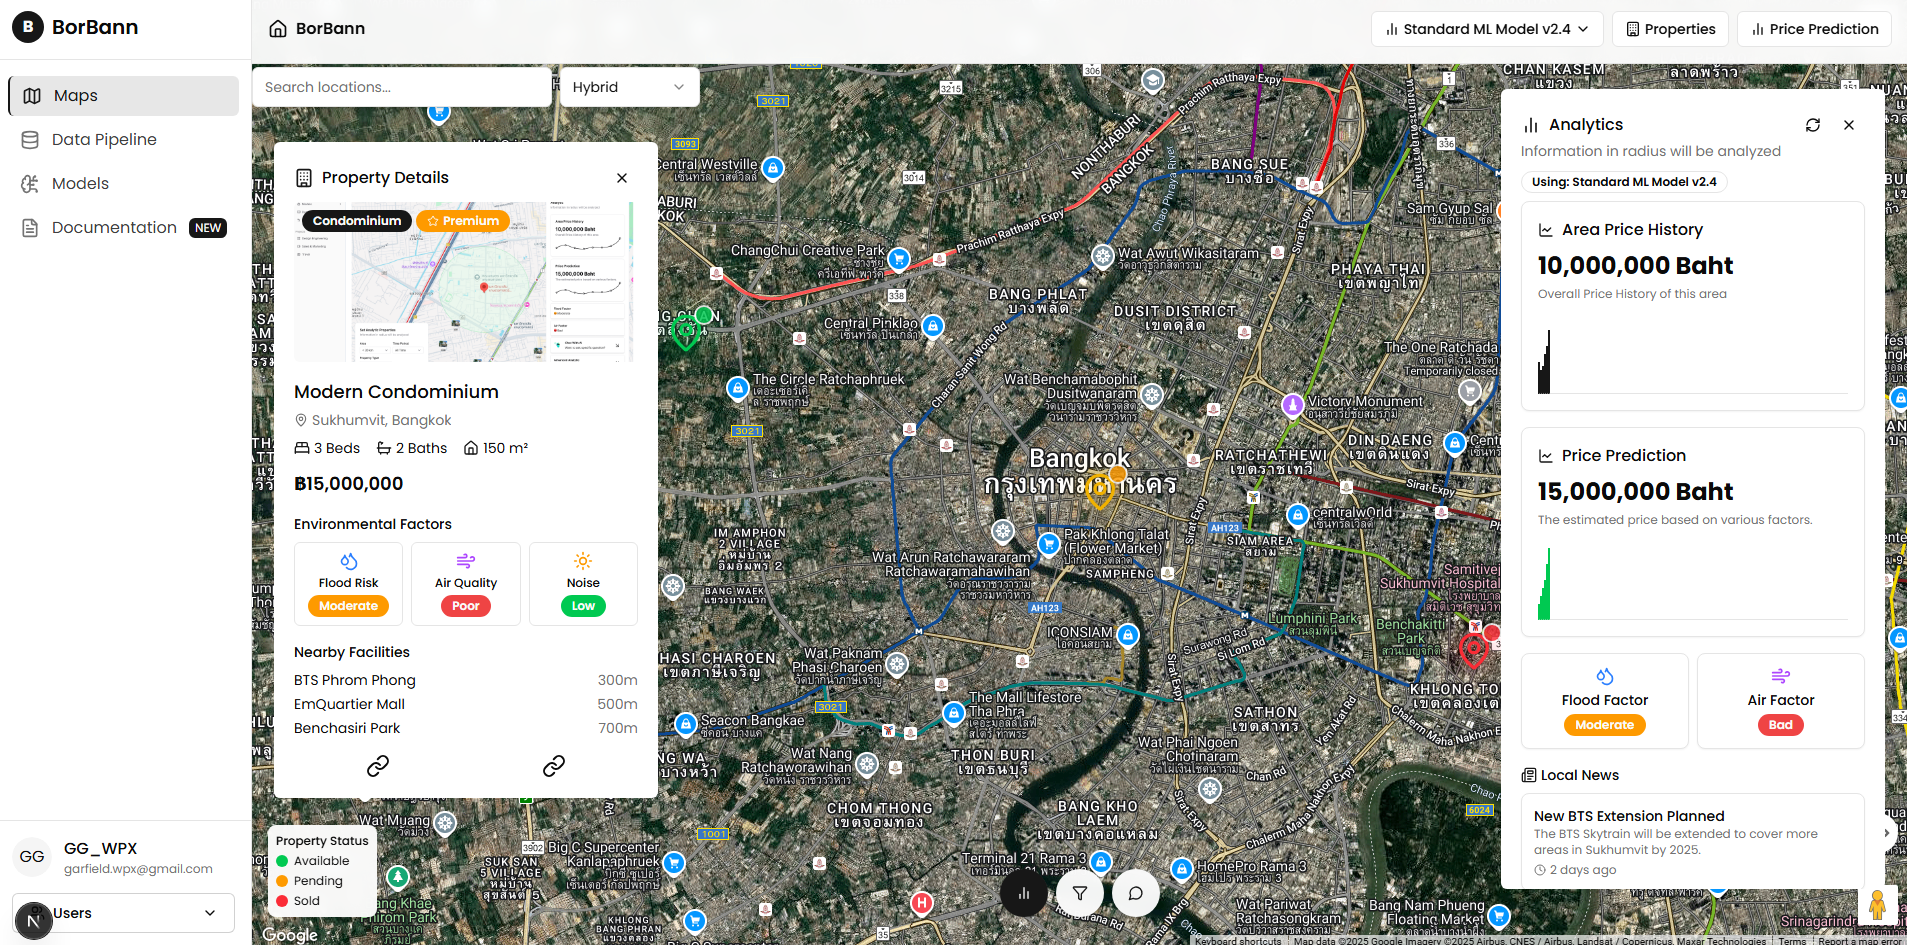
\includegraphics[width=1\textwidth]{assets/ai/insight-1.png}
	\caption{Environmental Impact Analysis}
	\label{fig:insight-ui-1}
\end{figure}

Figure \ref{fig:insight-ui-1} shows the analytics interface consisting of environmental data, pricing, and property-specific details along with nearby facilities.

\subsection{Explainable Price Prediction}

This feature blends predictive modeling with real-time visualizations and natural language explanations. Unlike typical black-box systems, BorBann’s model lets users interact with the logic behind the number. Users can explore, adjust, and challenge the AI's assumptions.

The user experience combines:

\begin{itemize}
	\item \textbf{Annotate} – each prediction includes visual and textual breakdowns of contributing factors.
	\item \textbf{Prompt} – the system suggests related factors for simulating “what-if” scenarios.
	\item \textbf{Automate} – the system recalibrates predictions as more data is integrated.
\end{itemize}

\subsubsection*{1. Prediction Overview}

When a user selects a property, the system immediately displays:

\begin{itemize}
	\item Predicted price range (upper and lower bounds)
	\item Confidence interval
	\item Base prediction with timestamp of latest data sync
\end{itemize}

\begin{figure}[htbp]
	\centering
	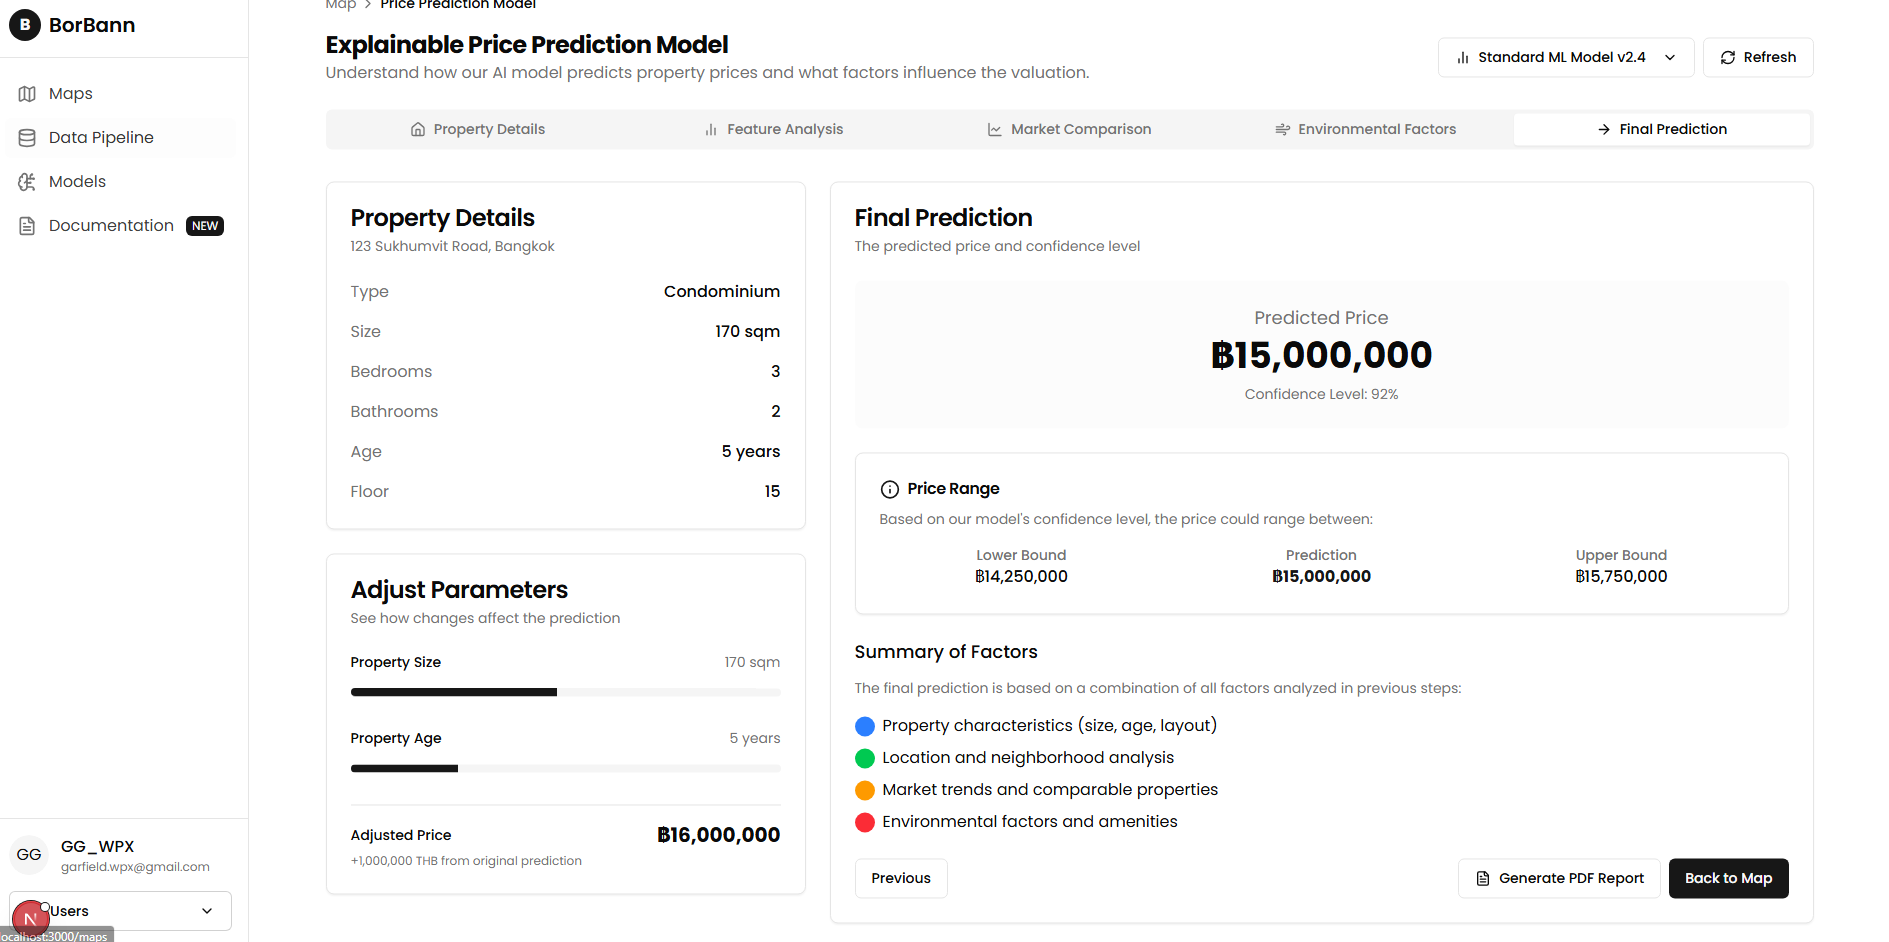
\includegraphics[width=1\textwidth]{assets/ai/price-prediction-1.png}
	\caption{Prediction Overview Interface}
	\label{fig:price-prediction-ui-1}
\end{figure}

Figure \ref{fig:price-prediction-ui-1} shows the price range, confidence bands, and a clean summary layout.

\subsubsection*{2. Feature Contribution Analysis}

The system explains which factors influenced the prediction most — such as location, property size, developer reputation, and local context.

\begin{figure}[htbp]
	\centering
	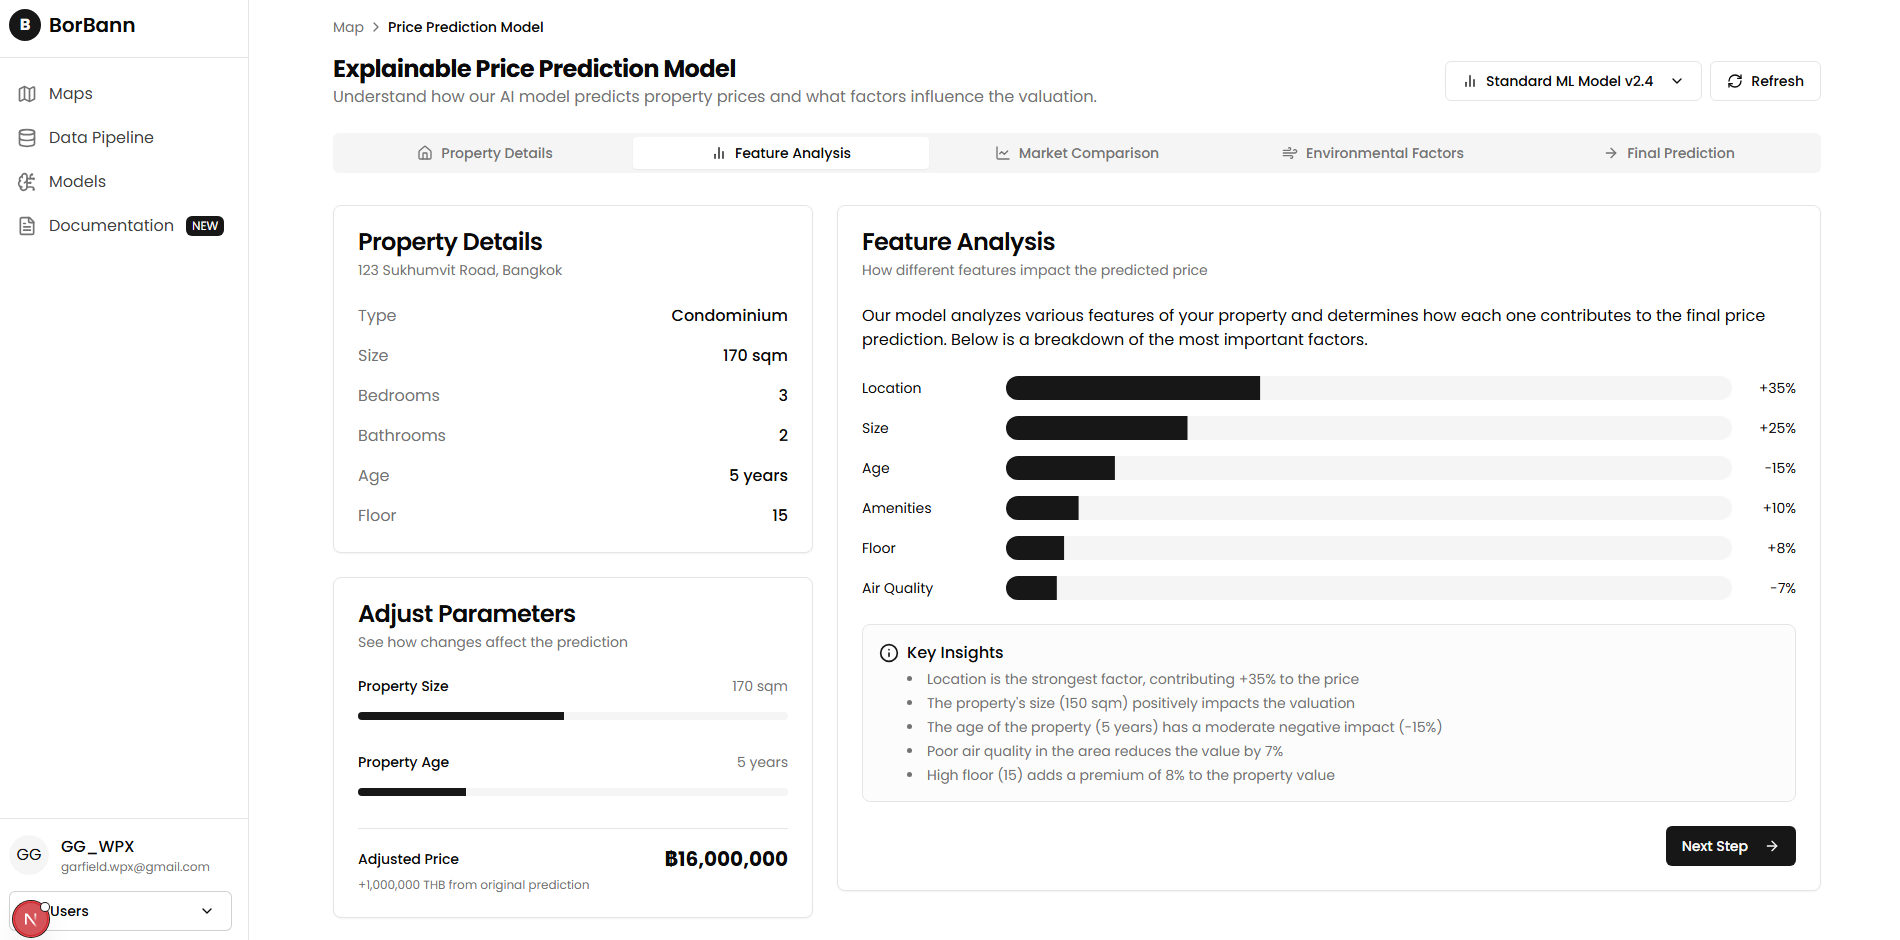
\includegraphics[width=1\textwidth]{assets/ai/price-prediction-2.png}
	\caption{Feature Contribution Analysis Interface}
	\label{fig:price-prediction-ui-2}
\end{figure}

Figure \ref{fig:price-prediction-ui-2} shows an interface that visualizes the impact of each factor using bar graphs and percentage values.


\section{Deployment Strategy}
\label{sec:deployment_strategy}

\subsection{Objective}
To detail the plan for integrating and running the AI-powered Real Estate Data Mapping model within a production environment, ensuring it effectively connects with the existing data ingestion pipeline and provides reliable, scalable, and maintainable operation. The AI model is central to transforming heterogeneous source data (from APIs, files, and web scraping) into a unified canonical format for real estate listings.

\subsection{Deployment Plan}

\subsubsection{Chosen Environment: Cloud-Based Deployment}
The AI model, along with the entire data integration pipeline system, will be deployed on a \textbf{Cloud Platform} which is Google Cloud Platform (GCP). Vary between each AI component, for example, data schema mapping will use Vertex AI while other may use cloud computing.

\textbf{Justification:}
\begin{itemize}
    \item \textbf{Scalability:} Cloud platforms offer elastic scaling of compute resources (CPUs, GPUs for LLM inference) and managed services, crucial for handling variable data loads and complex model computations.
    \item \textbf{Managed Services:} Leveraging services like Kubernetes (GKE, EKS, AKS) for container orchestration, managed databases for storing pipeline configurations and results, object storage (GCS, S3) for raw data and model artifacts, and potentially managed AI platforms (Vertex AI, SageMaker) simplifies infrastructure management.
    \item \textbf{Reliability \& Availability:} Cloud providers offer high availability zones and built-in redundancy features.
    \item \textbf{Integration:} Easier integration with other cloud services (e.g., data warehouses, monitoring tools).
\end{itemize}
While on-device or embedded systems are not suitable for this large-scale data processing and LLM inference task, an Edge deployment could be considered in the future for specific data pre-processing or localized data collection components if required, but the core AI mapping will reside in the cloud.

\subsubsection{AI Communication with the System: Internal Service Integration}
The AI mapping model will not be exposed as a standalone, public-facing API initially. Instead, it will be integrated as an internal component within the existing data integration pipeline's backend service (built with FastAPI).

\textbf{Communication Flow:}
\begin{enumerate}
    \item The \texttt{PipelineService} in the FastAPI application receives a request to run a specific pipeline (e.g., via its existing API endpoint \texttt{/pipelines/\{pipeline\_id\}/run}).
    \item If the pipeline configuration specifies the \texttt{ML\_MAPPING} strategy, the \texttt{PipelineService} invokes the \texttt{IngestionStrategyFactory}.
    \item The factory instantiates the \texttt{MLIngestionStrategy} (or a specialized version like \texttt{VertexAIMappingStrategy}).
    \item The \texttt{MLIngestionStrategy} internally:
        \begin{itemize}
            \item Loads or accesses the pre-trained/fine-tuned classification model (to identify real estate listings).
            \item Loads or accesses the pre-trained/fine-tuned LLM mapping model (e.g., from an MLflow registry, a local path within the container, or by calling a managed AI service like Vertex AI).
            \item Processes the input \texttt{AdapterRecord} data.
            \item Returns the mapped \texttt{CanonicalRecord} objects (as \texttt{OutputData}) back to the \texttt{PipelineService}.
        \end{itemize}
    \item The \texttt{PipelineService} then stores these results.
\end{enumerate}
This internal integration ensures that the AI model is a processing step within a larger workflow, rather than a standalone service that other parts of the system call directly via network requests for each mapping task. If a dedicated, reusable mapping service is needed later, a gRPC or REST API wrapper around the core mapping logic could be developed.

\subsubsection{Tools and Frameworks Used}
\begin{itemize}
    \item \textbf{FastAPI:} For the main backend service orchestrating pipelines and exposing management APIs.
    \item \textbf{Python:} Primary programming language for the backend and AI model implementation.
    \item \textbf{Google Cloud Vertex AI} For using pre-trained foundation models (e.g., Gemini), fine-tuning models via Generative AI Studio, and deploying them as managed endpoints. Communication would be via the Google Cloud Python client libraries.
    \item \textbf{Pydantic:} For data validation of input, intermediate, and canonical schemas.
    \item \textbf{Loguru:} For structured logging throughout the application and AI components.
    \item \textbf{Cloud Storage (GCS, S3):} For storing raw input data, training datasets, and large model artifacts.
    \item \textbf{SQLite} For storing pipeline configurations, run metadata, and potentially links to canonical data results.
\end{itemize}

\subsubsection{System Characteristics}
\textbf{Reliability:}
\begin{itemize}
    \item \textbf{Error Handling \& Retries:}
        \begin{itemize}
            \item The \texttt{PipelineService} will implement robust error handling for ingestion strategy failures (including AI model errors).
            \item For transient issues (e.g., temporary unavailability of a cloud AI service), retry mechanisms (e.g., using libraries like `tenacity`) will be implemented for external API calls made by the \texttt{MLIngestionStrategy}.
            \item The scheduler (APScheduler) has misfire grace time configurations.
        \end{itemize}
    \item \textbf{Input Validation:} Pydantic validation at multiple stages (API input, canonical output) ensures data integrity.
\end{itemize}

\textbf{Security:}
\begin{itemize}
    \item \textbf{Cloud IAM:} Utilize cloud provider Identity and Access Management (IAM) for granular control over access to resources (databases, storage, AI services, Kubernetes cluster). Principle of least privilege will be applied.
    \item \textbf{Secrets Management:} API keys for external LLMs (if used), database credentials, and other secrets will be managed using a secure secrets manager (e.g., HashiCorp Vault, Google Secret Manager, AWS Secrets Manager) and injected into containers as environment variables or mounted volumes, not hardcoded.
    \item \textbf{Data Encryption:} Data at rest (Cloud Storage, Databases) and in transit (HTTPS for external APIs, internal VPC traffic) will be encrypted.
\end{itemize}

\textbf{Maintainability \& Scalability:}
\begin{itemize}
    \item \textbf{Modular Design:} The separation of concerns (\texttt{PipelineService}, \texttt{IngestionStrategyFactory}, specific \texttt{Strategy} classes) allows for independent updates and maintenance of components.
    \item \textbf{Comprehensive Logging (Loguru):} Structured logs are centralized (e.g., Google Cloud Logging, ELK stack) for easier debugging and monitoring. The SSE log streaming endpoint aids real-time monitoring of specific pipeline runs.
    \item \textbf{Scalability (Application):} Kubernetes Horizontal Pod Autoscaler (HPA) will automatically scale the number of FastAPI application pods based on CPU/memory utilization or custom metrics.
    \item \textbf{Scalability (AI Model Inference):}
        \begin{itemize}
            \item \textbf{Managed AI Service (e.g., Vertex AI):} These services typically handle autoscaling of the model endpoint based on traffic. Configure appropriate instance types and min/max replica counts.
        \end{itemize}
\end{itemize}

\subsection{Proof of Concept}
\label{ssec:poc}

\subsubsection{AI Model Build and Test Process}
The AI model for mapping real estate data to the \texttt{CanonicalRecord} schema was developed iteratively, focusing initially on an LLM-based approach.

\textbf{Development Stages}
\begin{enumerate}
    \item \textbf{Data Collection \& Annotation}

    A diverse dataset of approximately 500 property records was collected from various sources, including:
    \begin{itemize}
        \item Simulated API outputs (e.g., mock property APIs)
        \item Example CSV/JSON datasets
        \item Real estate websites such as Baania and Zillow (conceptual scraping)
    \end{itemize}

    These records were manually mapped to a unified schema called \texttt{CanonicalRecord}. A foundation model (e.g., GPT-4) was used to generate initial prompt-completion pairs via meta-prompting. All completions were manually reviewed and corrected to produce high-quality training data.

    \item \textbf{LLM Mapper Fine-Tuning (Primary Task)}

    \begin{itemize}
        \item \textbf{Model Selection:} Experiments were conducted on gemini-2.0-flash-lite-001.
        \item \textbf{Fine-Tuning Strategy:} Fine-Tuning with supervised method on Vertex AI platform.
        \item \textbf{Training Data:} About 30 prompt-completion pairs were used with 10 data point for evaluation set. Each prompt contained instructions, the full schema, and raw data. Each completion was a valid JSON object adhering to the \texttt{CanonicalRecord} structure.
        \item \textbf{Platform:} All tuning jobs were executed on Vertex AI.
            \begin{itemize}
                \item Hyperparameters: base model, learning rate, batch size, LoRA rank, LoRA alpha, and epoch count.
                \item Outputs: Adapter weights, tokenizer config, and example outputs on the eval set.
            \end{itemize}
    \end{itemize}

    \item \textbf{Evaluation Methodology}

    \begin{itemize}
        \item \textbf{During Fine-Tuning:} Vertex AI provides training and validation losses automatically when an eval set is supplied.
        \item \textbf{Post Fine-Tuning:}
            \begin{itemize}
                \item \textbf{JSON Syntactic Validity:} Parse output strings using \texttt{json.loads()}.
                \item \textbf{Pydantic Schema Conformance:} Instantiate \texttt{CanonicalRecord(**parsed\_json)} to verify structural correctness.
            \end{itemize}
        \item \textbf{Manual Review:} A qualitative check was performed to ensure logical accuracy and edge case handling in LLM outputs.
    \end{itemize}
\end{enumerate}


\subsubsection{Model Performance Results}
Performance metrics are based on 2 metrics:
        \begin{itemize}
            \item \textbf{JSON Syntactic Validity}: Parse the output string and check for validity.
            \item \textbf{Pydantic Schema Conformance}: Check with pre-defined pydantic schema to ensure that it output the desire data scheme.
        \end{itemize}

\begin{table}[htbp]
    \centering
    \caption{Pipeline Validation Metrics}
    \label{tab:pipeline_validation_metrics}
    \begin{tabular}{llc}
        \toprule
        \textbf{Model Version} & \textbf{Metric} & \textbf{Value (\%)} \\
        \midrule
        \textbf{BORBANN\_PIPELINE\_2} 
            & JSON Syntactic Validity & 91.67\% \\
            & Pydantic Schema Conformance & 63.64\% \\
        \midrule
        \textbf{BORBANN\_PIPELINE\_3} 
            & JSON Syntactic Validity & 100.00\% \\
            & Pydantic Schema Conformance & 0.00\% \\
        \midrule
        \textbf{BORBANN\_PIPELINE\_4} 
            & JSON Syntactic Validity & 100.00\% \\
            & Pydantic Schema Conformance & 0.00\% \\
        \bottomrule
    \end{tabular}
\end{table}


Table~\ref{tab:pipeline_validation_metrics} presents the validation performance of three pipeline variants. Among them, \texttt{borbann-pipeline-2} achieves the highest score in JSON syntactic validity (91.67\%), indicating that it produces well-formed JSON outputs most consistently. However, it performs best in this metric while showing only moderate conformance to the Pydantic schema (63.64\%).

In contrast, both \texttt{borbann-pipeline-3} and \texttt{borbann-pipeline-4} attain perfect JSON syntactic validity (100\%) but fail completely in Pydantic schema conformance (0.00\%). This suggests that although their outputs are syntactically correct, they do not adhere to the expected canonical data structure.

Based on this evaluation, we select \texttt{borbann-pipeline-2} as the final model for deployment. The superior schema adherence—despite not being perfect—makes it more suitable for downstream structured processing tasks.

A possible reason for the low schema conformance in pipelines 3 and 4 may be suboptimal prompt design during fine-tuning. The model may have overfit to an incorrect or inconsistent output structure due to insufficient coverage of schema variations in the training data. This highlights the importance of prompt engineering and data diversity when fine-tuning large language models for structured output tasks.
